\documentclass{standalone}

\usepackage{tikz}
\usetikzlibrary{angles,quotes}
\usepackage{amsmath,amssymb,amsfonts}

\usepackage{pgfplots}
\definecolor{darkgreen}{rgb}{0.0, 0.42, 0.24}
\definecolor{amethyst}{rgb}{0.6, 0.4, 0.8}

\pgfplotsset{compat=newest}
\pgfplotsset{every axis/.append style={
                     tick label style={font=\footnotesize},
                 }}


\begin{document}
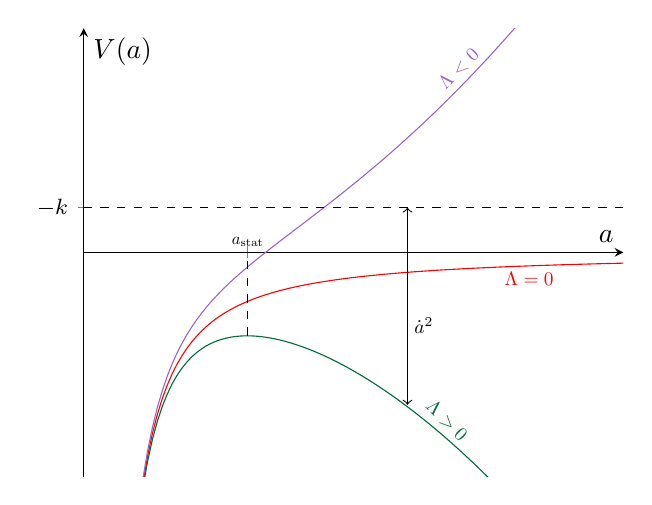
\begin{tikzpicture}
 \begin{axis}[axis lines =center,xmin=0,xmax=5,ymin=-5,ymax=5,
 xtick={1.52},
 xticklabels={},
 ytick={0,1},
 yticklabels={0,$-k$},
 xlabel=$a$,ylabel=$V(a)$,
 legend style={nodes={scale=0.6, transform shape}}]
 
    \addplot[color=darkgreen,samples=100,domain=0.5:5]{(-1/x^2)-(1/x)-(1/3)*1*x^2} node[above,pos=0.6,scale=0.7,rotate={-45}]{$\Lambda>0$};
     \addplot[color=red,samples=100,domain=0.5:5]{(-1/x^2)-(1/x)-(1/3)*0*x^2}node[below,pos=0.9,scale=0.7]{$\Lambda=0$};;
      \addplot[color=amethyst,samples=100,domain=0.5:5]{(-1/x^2)-(1/x)+(1/3)*1*x^2}node[above,pos=0.7,scale=0.7,rotate={45}]{$\Lambda<0$};;
      \addplot[dashed](0,1)--(5,1);
      \addplot[dashed](1.52,-1.86)--(1.52,0) node[above,pos=1,scale=0.6]{$a_{\text{stat}}$};
      \draw[<->,thin](3,1)--(3,-3.4) node[right,pos=0.6,scale=0.7]{$\dot{a}^2$};
    
 \end{axis}

\end{tikzpicture}
\end{document}